\documentclass[11pt]{article}
\usepackage{fontspec}
\usepackage[a4paper,margin=2.3cm]{geometry}
\usepackage{graphicx}
\usepackage{booktabs}
\usepackage{array}
\usepackage{xcolor}
\usepackage{float}
\usepackage{fancyvrb}
\usepackage[hidelinks]{hyperref}

\setmainfont{Helvetica Neue}
\setmonofont{Menlo}
\renewcommand{\arraystretch}{1.25}

\title{\textbf{Athena TTS — Báo cáo sơ bộ}\\[2pt]
\large So sánh 5 engine TTS mã nguồn mở}
\author{}
\date{15/06/2026}

\begin{document}
\maketitle
\vspace{-1.5em}

\section*{1. Tổng quan}
Cùng một đoạn kịch bản tiếng Anh (9 câu) được đưa qua 5 engine TTS. Bốn engine có
nhân bản giọng dùng chung một file mẫu \texttt{refs/speaker.wav} (11 giây); Kokoro
dùng giọng cài sẵn. Tất cả chạy trên CPU (Apple M4 Pro).

\section*{2. Kịch bản được test}
\begin{Verbatim}[frame=single,fontsize=\small,rulecolor=\color{gray}]
Hello, this is a short voice consistency test.
Please keep the same tone, speed, and energy throughout the recording.
The quick brown fox jumps over the lazy dog.
Today is June fifteenth, twenty twenty-six.
I will now repeat one sentence three times.
The product sounds clear, stable, and natural.
The product sounds clear, stable, and natural.
The product sounds clear, stable, and natural.
End of test. Thank you.
\end{Verbatim}
\noindent Kịch bản cố ý lặp 1 câu 3 lần để kiểm tra \textit{tính nhất quán} của giọng
(tone, tốc độ, năng lượng) giữa các lần đọc giống nhau.

\section*{3. Cơ chế từng engine (tóm tắt)}
\begin{table}[H]\centering\small
\begin{tabular}{>{\bfseries}l l p{9.2cm}}
\toprule
Engine & Kiểu & Cơ chế (đơn giản) \\
\midrule
Kokoro & Non-autoreg. (82M) & Mô hình nhỏ, sinh thẳng một lần. Giọng cài sẵn (style vector). Không nhân bản giọng $\rightarrow$ nhanh nhất. \\
Chatterbox & Tự hồi quy (LM) & Transformer kiểu Llama (0.5B) sinh ``token âm thanh'' lần lượt từ văn bản + giọng mẫu, rồi vocoder dựng sóng. Có điều khiển cảm xúc. \\
F5-TTS & Flow-matching (DiT) & Diffusion Transformer, sinh song song. ``Điền'' phần giọng còn thiếu dựa trên audio mẫu + văn bản qua nhiều bước; vocoder Vocos. \\
StyleTTS2 & Style diffusion + GAN & Diffusion sinh ``style vector'', kèm bộ dự đoán thời lượng/ngữ điệu và decoder kiểu HiFi-GAN; huấn luyện đối kháng. Nhân bản zero-shot. \\
IndexTTS2 & Tự hồi quy (GPT) & GPT sinh token ngữ nghĩa; dùng semantic codec (w2v-BERT + MaskGCT), embedding người nói (CAMPPlus), cảm xúc (Qwen), rồi flow $\rightarrow$ mel + vocoder BigVGAN. \\
\bottomrule
\end{tabular}
\end{table}

\section*{4. Thời gian tạo (CPU, model đã cache)}
Đo tuần tự (không chạy song song) để tránh tranh CPU; gồm thời gian nạp model + suy luận.
\begin{table}[H]\centering
\begin{tabular}{l r r}
\toprule
Engine & Thời gian (giây) & Độ dài audio (giây) \\
\midrule
Kokoro     & 12.7  & 29.4 \\
StyleTTS2  & 29.5  & 39.4 \\
Chatterbox & 38.0  & 33.4 \\
IndexTTS2  & 68.8  & 25.2 \\
F5-TTS     & 253.7 & 37.4 \\
\bottomrule
\end{tabular}
\end{table}
\noindent\textit{Ghi chú:} lần chạy đầu tiên còn phải tải model (Index $\sim$6\,GB, F5 $\sim$1.3\,GB\dots) nên lâu hơn nhiều; bảng trên là thời gian khi đã có sẵn model.

\section*{5. Đánh giá độ ``người'' (chỉ số khách quan)}
Các tiêu chí: \textit{ngữ điệu/luyến láy} (dao động cao độ theo semitone), \textit{cao--thấp}
(khoảng F0), \textit{tự nhiên} (biến thiên năng lượng, ngắt nghỉ), \textit{tone giọng} (timbre).
Điểm càng cao càng giống người.
\begin{table}[H]\centering
\begin{tabular}{c >{\bfseries}l r p{7.5cm}}
\toprule
\# & Engine & Điểm & Nhận xét \\
\midrule
1 & StyleTTS2  & 89.6 & Cân bằng tốt nhất: ngữ điệu mượt, cao độ tự nhiên, ổn định. \\
2 & IndexTTS2  & 89.5 & Biểu cảm nhất, luyến láy phong phú, timbre ấm; sát nút. \\
3 & Kokoro     & 80.9 & Tự nhiên và nhanh, nhưng giọng hơi sáng/gắt. \\
4 & Chatterbox & 78.4 & Dao động cao độ rộng nhưng hơi cao, kém ổn định một chút. \\
5 & F5-TTS     & 35.4 & Cao độ mất ổn định (dao động loạn) nên nghe ``máy'' hơn. \\
\bottomrule
\end{tabular}
\end{table}

\begin{figure}[H]\centering
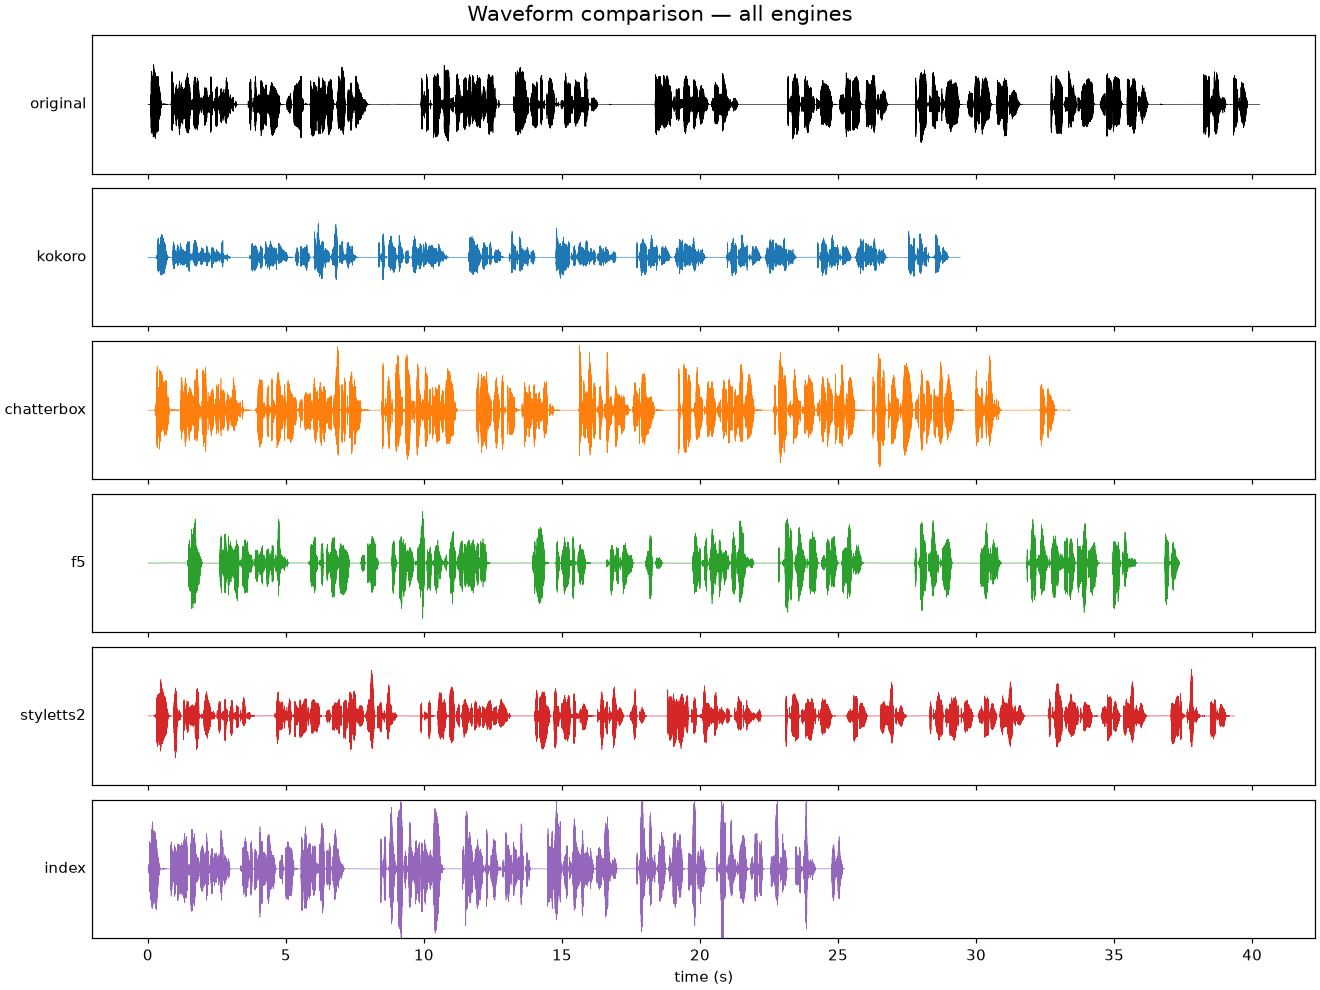
\includegraphics[width=\linewidth]{compare_waveforms.png}
\caption{Biểu đồ sóng của 5 engine trên cùng kịch bản.}
\end{figure}

\begin{figure}[H]\centering
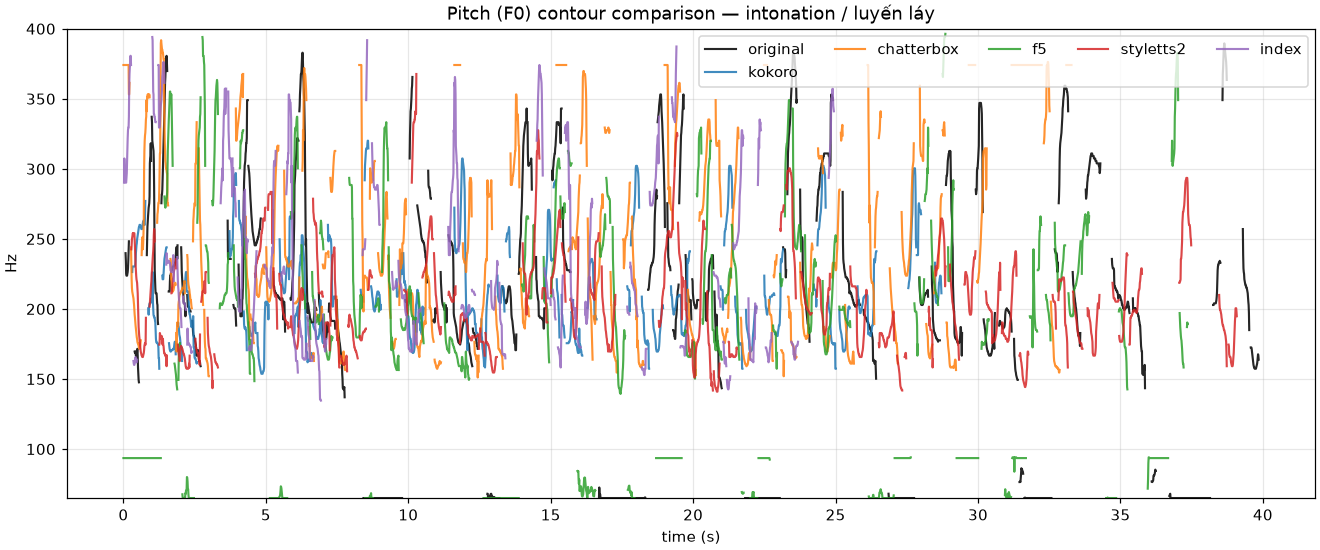
\includegraphics[width=\linewidth]{compare_pitch.png}
\caption{Đường cao độ (F0) chồng nhau — thể hiện ngữ điệu/luyến láy. F5 dao động loạn nhất.}
\end{figure}

\section*{6. Ưu / nhược điểm từng engine}
\begin{table}[H]\centering\small
\begin{tabular}{>{\bfseries}l p{5.6cm} p{5.6cm}}
\toprule
Engine & Ưu điểm & Nhược điểm \\
\midrule
Kokoro & Nhanh nhất ($\sim$real-time); setup dễ nhất; nhẹ (82M); license thoáng; ổn định. & \textbf{Không nhân bản giọng} (chỉ giọng cài sẵn); ít biểu cảm; timbre hơi sáng/gắt. \\
Chatterbox & Nhân bản giọng tốt; có điều khiển cảm xúc; chất lượng khá; setup tương đối dễ. & Tự hồi quy nên chậm hơn; cao độ hơi cao + kém ổn định chút; kéo lùi phiên bản torch. \\
F5-TTS & Clone giọng mạnh kiểu in-context; có sẵn CLI; giọng rõ. & \textbf{Chậm nhất trên CPU} ($\sim$4 phút); cao độ mất ổn định; cần cả mẫu + transcript; deps nặng. \\
StyleTTS2 & \textbf{Tự nhiên nhất}; nhanh khá; clone zero-shot tốt. & Không có CLI chính thức (phải tự viết script); checkpoint cũ (cần vá \texttt{torch.load}); phải trỏ espeak thủ công. \\
IndexTTS2 & Biểu cảm nhất; \textbf{điều khiển cảm xúc + thời lượng}; clone zero-shot; timbre ấm. & \textbf{Nặng nhất} ($\sim$10\,GB + tải thêm lúc chạy); setup phức tạp ($uv$, Python 3.10 riêng); ngốn RAM. \\
\bottomrule
\end{tabular}
\end{table}

\noindent\textbf{Gợi ý chọn:} cần nhanh/nhẹ, không clone $\rightarrow$ \textbf{Kokoro};
tự nhiên nhất kèm clone $\rightarrow$ \textbf{StyleTTS2};
biểu cảm + điều khiển cảm xúc $\rightarrow$ \textbf{IndexTTS2};
clone dễ, ít setup $\rightarrow$ \textbf{Chatterbox};
F5-TTS chỉ nên dùng khi có GPU.

\section*{7. Kết luận}
\textbf{StyleTTS2} và \textbf{IndexTTS2} cho giọng tự nhiên (``người'') nhất, gần ngang nhau:
StyleTTS2 mượt và ổn định hơn, IndexTTS2 biểu cảm hơn. \textbf{Kokoro} nhanh nhất và đủ tốt
nhưng giọng hơi sáng. \textbf{F5-TTS} có cao độ kém ổn định nên nghe ``máy'' hơn.
\textit{Lưu ý:} đây là chỉ số khách quan gián tiếp, nên nghe trực tiếp để xác nhận.

\end{document}
